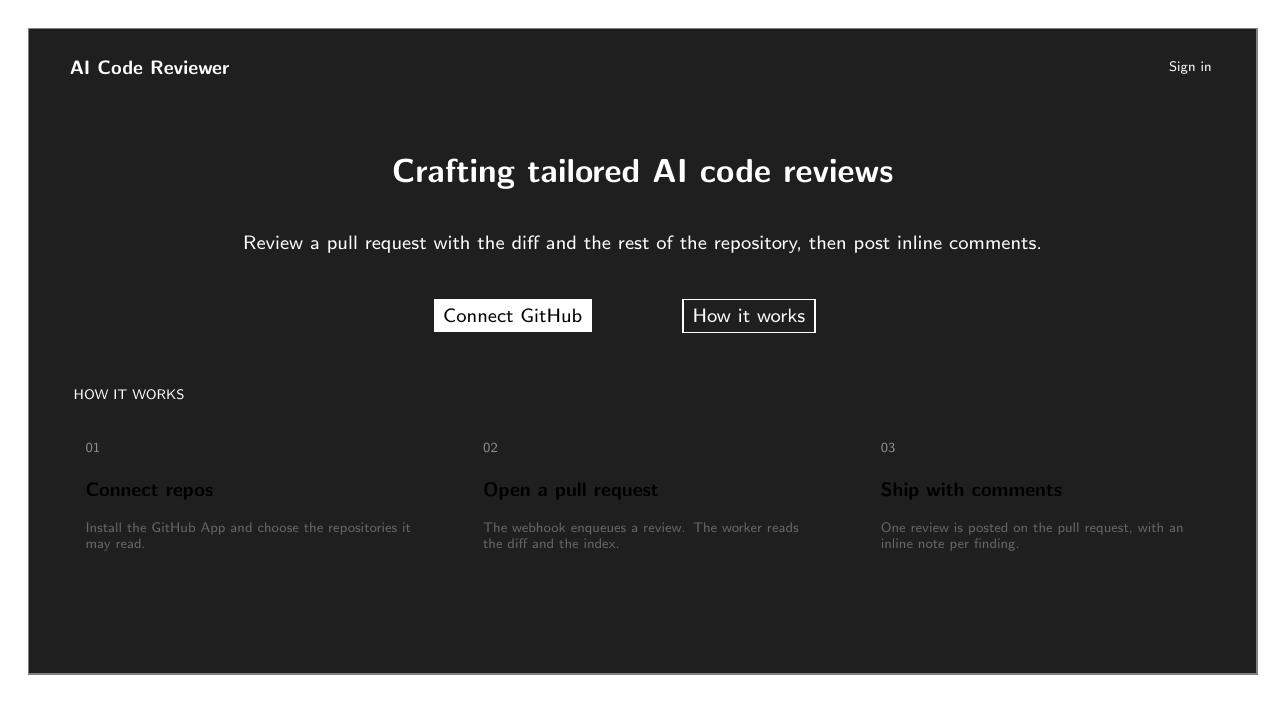
\begin{tikzpicture}[x=1cm,y=1cm]
  \fill[black!88] (0,0) rectangle (15.6,8.2);
  \draw[black!50, line width=0.6pt] (0,0) rectangle (15.6,8.2);

  \node[anchor=west, font=\sffamily\bfseries\scriptsize, text=white] at (0.4,7.7) {AI Code Reviewer};
  \node[anchor=east, font=\sffamily\tiny, text=white!75] at (15.15,7.7) {Sign in};

  \node[align=center, font=\sffamily\bfseries\large, text=white, text width=12cm] at (7.8,6.35)
    {Crafting tailored AI code reviews};
  \node[align=center, font=\sffamily\scriptsize, text=white!65, text width=11cm] at (7.8,5.45)
    {Review a pull request with the diff and the rest of the repository, then post inline comments.};

  \node[fill=white, font=\sffamily\scriptsize, inner sep=3.5pt] at (6.15,4.55) {Connect GitHub};
  \node[draw=white!50, font=\sffamily\scriptsize, text=white, inner sep=3.5pt] at (9.15,4.55) {How it works};

  \node[anchor=west, font=\sffamily\tiny, text=white!50] at (0.45,3.55) {HOW IT WORKS};

  \wfpanel{0.4}{0.4}{4.7}{2.85}
  \node[anchor=north west, font=\sffamily\tiny, text=black!45] at (0.6,3.05) {01};
  \node[anchor=north west, font=\sffamily\bfseries\scriptsize] at (0.6,2.55) {Connect repos};
  \node[anchor=north west, font=\sffamily\tiny, text=black!60, text width=4.2cm] at (0.6,2.05)
    {Install the GitHub App and choose the repositories it may read.};

  \wfpanel{5.45}{0.4}{4.7}{2.85}
  \node[anchor=north west, font=\sffamily\tiny, text=black!45] at (5.65,3.05) {02};
  \node[anchor=north west, font=\sffamily\bfseries\scriptsize] at (5.65,2.55) {Open a pull request};
  \node[anchor=north west, font=\sffamily\tiny, text=black!60, text width=4.2cm] at (5.65,2.05)
    {The webhook enqueues a review. The worker reads the diff and the index.};

  \wfpanel{10.5}{0.4}{4.7}{2.85}
  \node[anchor=north west, font=\sffamily\tiny, text=black!45] at (10.7,3.05) {03};
  \node[anchor=north west, font=\sffamily\bfseries\scriptsize] at (10.7,2.55) {Ship with comments};
  \node[anchor=north west, font=\sffamily\tiny, text=black!60, text width=4.2cm] at (10.7,2.05)
    {One review is posted on the pull request, with an inline note per finding.};
\end{tikzpicture}
